\section{Introducción}

En los últimos años, la evolución en el campo de la industria ha sido tan grande que ha llegado al punto que se ha hecho necesario el desarrollo de robots para poder realizar las tareas de manera más eficaz, eficiente y segura. Estos robots pueden tener diferente apariencia y función según el ámbito al que se apliquen, desde robots industriales hasta robots para las tareas domésticas. En el campo industrial los robots pueden ser más simples ya que el entorno es principalmente estático, las tareas a desarrollar son repetitivas y automáticas, y apenas hay interacción humana. 

Pero no todos los entornos reúnen las condiciones ideales de ser estáticos y repetitivos. Por esta razón surgió la necesidad de crear robots que fueran capaces de trabajar en entornos dinámicos siendo capaces de desarrollar tareas complejas e interactuar con los seres humanos y su entorno. De esa idea de interacción humana surgieron los robots humanoides, con forma humana e inteligencia artificial, que les permite desarrollar un comportamiento y acciones más parecidas a las de los humanos. Pero para llevar a cabo esas acciones es necesario un control ya que la posibilidad de moverse trae consigo el problema de la estabilidad.

\begin{figure}[H]
\centering
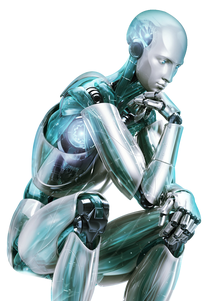
\includegraphics[scale=0.7]{imagenes/apartado_1/11_robot_humanoide}
\caption{Robot humanoide}
\label{figura1}
\end{figure}
%% Imagen sacada de https://sourcingguy.wordpress.com/2015/09/16/managing-procurement-in-a-digital-world/

Evitar la pérdida de equilibrio del robot durante las fases de posición estática o caminata bípeda es una tarea compleja que está relacionada con el control.

Además, pueden aparecer perturbaciones que dificulten el equilibrio. Dichas perturbaciones pueden surgir de diversas fuentes como pueden ser un empujón o un terreno irregular. El ser humano es capaz de corregirlas inconscientemente moviendo el cuerpo o cualquier articulación. Este movimiento no lo realizan los robots por sí solos por lo que para lograrlo éstos deben imitar nuestros patrones a través de la programación que se les ha proporcionado para estabilizarse por sí solos. 


\subsection{Motivaciones y origen del proyecto}

En la actualidad uno de los campos con mayor proyección en la investigación dentro del campo de la robótica es el de crear un robot capaz de desenvolverse por sí solo en el entorno de los seres humanos. De esta idea nacen los robots humanoides, robots con apariencia de ser humano que con inteligencia artificial pretenden mimetizar nuestros comportamientos para desenvolverse en entornos similares al nuestro.

La investigación ha avanzado mucho en  los últimos años debido al avance tecnológico en el que nos encontramos. 

Pero éstos tienen un problema, la estabilidad al realizar movimientos. Han surgido diversos estudios acerca de aproximarse lo máximo posible a la idea de estabilización del robot, pero dichos estudios poseen diferentes salidas debido a las interferencias de los sensores y el entorno. 

De aquí surgió la idea del actual proyecto, en el que se pretende mejorar la respuesta de los sensores, reduciendo el error, ante estímulos externos para así poder aumentar la estabilidad del robot humanoide TEO.

\subsection{Objetivos}

Este proyecto trata sobre el estudio de estabilidad del robot humanoide TEO haciendo uso de la información recibida de los diferentes sensores que posee, tanto los de fuerza-par como el inercial.

Los objetivos del presente trabajo son:

- Realizar un estudio de estabilidad a través de los diferentes modelos existentes, como son el modelo de péndulo invertido y el cart-table.

- Desarrollar un control que reduzca el error del modelo de péndulo invertido y así conseguir que el ZMP práctico y el ZMP teórico coincidan.

- Desarrollar un modelo predictivo que actúe ante perturbaciones externas mediante el uso del sensor inercial del robot TEO.

\subsection{Marco regulador}

%https://blogthinkbig.com/las-6-leyes-de-la-robotica-de-la-union-europea

Debido al aumento tanto de la tecnología como de la inteligencia artificial en nuestras vidas, las grandes organizaciones gubernamentales se han visto obligadas a redactar una serie de leyes que regulen la convivencia de los robots y los humanos. Se puede considerar como precursor de las normativas a Isaac Asimov, quien estableció las tres leyes principales que todo robot debe cumplir \cite{ref1}

\begin{enumerate}
\item Un robot no hará daño a un ser humano, ni permitirá con su inacción que sufra daño.
\item Un robot debe obedecer las órdenes dadas por un ser humano excepto si éstas entran en conflicto con la 1ª ley.
\item Un robot debe proteger su propia existencia en la medida en la que la protección no entre en conflicto con la 1ª y la 2ª ley.
\end{enumerate}
%
%
%http://www.aenor.es/aenor/normas/buscadornormas/buscadornormas.asp#.WwxD43WFM8p

Debido a la continua implantación de robots en el sector industrial y su interacción con seres humanos en un mismo espacio de trabajo, se redactaron una serie de leyes, entre las que se encuentran:
\begin{enumerate}
\item UNE-EN ISO 10218-1:2012 Robots y dispositivos robóticos. Requisitos de seguridad para robots industriales. Parte 1: Robots. (ISO 10218-1:2011).
\item UNE-EN ISO 10218-2:2011 Robots y dispositivos robóticos. Requisitos de seguridad para robots industriales. Parte 2: Sistemas robot e integración. (ISO 10218-2:2011).
\end{enumerate}

%http://www.infoplc.net/actualidad-industrial/item/103207-iso-norma-ts15066-robots-colaborativos
Estas leyes fueron concebidas para proporcionar unas pautas de seguridad en entornos en los que robot y humano comparten el mismo espacio de trabajo.

Fuera del ámbito industrial, la Unión Europea ha propuesto una serie de leyes para, en un futuro, poder regular la convivencia de robots y seres humanos en cualquier entorno:

\begin{enumerate}

\item ``Los robots deberán tener un interruptor de emergencia''

\item ``Los robots no podrán hacer daño a los seres humanos''

\item ``No podrán generarse relaciones emocionales con los robots''

\item ``Los que sean más grandes deberán tener un seguro obligatorio''

\item ``Derechos y obligaciones para los robots''

\item ``Tendrán la obligación de pagar impuestos''

\end{enumerate}


\subsection{Entorno socio-económico}

En este apartado se pretende mostrar un presupuesto general de dicho proyecto. Para llevarlo a cabo se han tenido en cuenta tanto los materiales utilizados como la mano de obra por parte de los participantes.

\begin{table}[H]
\begin{center}
\begin{tabular}{|c|c|c|c|c|}
\hline
\rowcolor[gray]{0.7}
\multicolumn{5}{|c|}{\textbf{COSTE MATERIAL}} \\ 
\hline
\rowcolor[gray]{0.9}
\textbf{Ítem} & \textbf{Descripción} & \textbf{\begin{tabular}[c]{@{}c@{}}Coste/ud\\ (\textup{\euro}/ud)\end{tabular}} & \textbf{Ud} & \textbf{\begin{tabular}[c]{@{}c@{}}Coste\\ (\textup{\euro})\end{tabular}} \\ 
\hline
1 & \multicolumn{1}{l|}{\begin{tabular}[c]{@{}l@{}}Ordenador Acer Aspire E1-571\\ \\ - Procesador Intel Core i3-2328M \\ (2,2GHz, 3MB L3 cache)\\ - Memoria RAM 6 DDR3\\ - Disco duro 500GB\\ - Monitor, Conexión ethernet y otros\end{tabular}} & 899 & 1 & 899 \\ 
\hline
2 & \begin{tabular}[c]{@{}c@{}}Sistema Operativo Linux \\ (Licencia gratuita)\end{tabular} & - & - & - \\ 
\hline
\multicolumn{1}{|c|}{3} & \multicolumn{1}{l|}{\begin{tabular}[c]{@{}l@{}}Programas (Licencia gratuita)\\ \\ - Python\\ - Qt Creator\end{tabular}} & \multicolumn{1}{c|}{-} & \multicolumn{1}{c|}{-} & \multicolumn{1}{c|}{-} \\ 
\hline
\multicolumn{1}{l}{} &  & \multicolumn{2}{c|}{\cellcolor[gray]{0.9}\textbf{TOTAL}} & \textbf{899\textup{\euro}} \\ \cline{3-5}
\hline
\rowcolor[gray]{0.7} 
\multicolumn{5}{|c|}{\textbf{COSTE LABORAL}} \\ 
\hline
\rowcolor[gray]{0.9} 
\multicolumn{1}{|c|}{\textbf{Ítem}} & \multicolumn{1}{c|}{\textbf{Descripción}} & \multicolumn{1}{c|}{\textbf{\begin{tabular}[c]{@{}c@{}}Coste/h\\ (\textup{\euro}/h)\end{tabular}}} & \multicolumn{1}{c|}{\textbf{Horas}} & \multicolumn{1}{c|}{\textbf{\begin{tabular}[c]{@{}c@{}}Coste\\ (\textup{\euro})\end{tabular}}} \\ 
\hline
\multicolumn{1}{|c|}{1} & \multicolumn{1}{l|}{\begin{tabular}[c]{@{}l@{}}\textbf{Tiempo dedicado proyectante}\\ \\ \\ - Desarrollo de algoritmos\\ (pruebas, programación,...)\\ - Memoria\end{tabular}} & \multicolumn{1}{c|}{\begin{tabular}[c]{@{}c@{}}\textbf{15}\\ \\ \\ 15\\ \\ 15\end{tabular}} & \multicolumn{1}{c|}{\begin{tabular}[c]{@{}c@{}}\textbf{370}\\ \\ \\ 250\\ \\ 120\end{tabular}} & \multicolumn{1}{c|}{\begin{tabular}[c]{@{}c@{}}5550\\ \\ \\ 3750\\ \\ 1800\end{tabular}} \\ 
\hline
\multicolumn{1}{|c|}{2} & \multicolumn{1}{l|}{\textbf{Tiempo tutorización}} & \multicolumn{1}{c|}{30} & \multicolumn{1}{c|}{80} & \multicolumn{1}{c|}{2400} \\ 
\hline
\multicolumn{1}{l}{} & \multicolumn{1}{l|}{} & \multicolumn{2}{c|}{\cellcolor[gray]{0.9}\textbf{TOTAL}} & \multicolumn{1}{c|}{\textbf{7950\textup{\euro}}} \\ 
\cline{3-5}
\end{tabular}
\end{center}
\caption{Presupuesto}
\label{tabla11}
\end{table}

\afterpage{\null\newpage}
\newpage

